\documentclass[11pt,a4paper]{article}

\usepackage[margin=2.2cm]{geometry}
\usepackage{amsmath,amssymb,amsthm,mathtools}
\usepackage[T1]{fontenc}
\usepackage[dvipsnames]{xcolor}
\usepackage{hyperref}
\usepackage{enumitem}
\usepackage[most]{tcolorbox}
\usepackage{tikz}
\usepackage{tkz-euclide}
\usetikzlibrary{arrows.meta}

\hypersetup{
  colorlinks=true,
  linkcolor=blue!55!black,
  urlcolor=blue!55!black
}

\setlist[enumerate]{itemsep=0.35em, topsep=0.45em}

\newtheorem{theorem}{Theorem}[section]
\newtheorem{definition}[theorem]{Definition}
\newtheorem{example}[theorem]{Example}
\newtheorem{remark}[theorem]{Remark}

\tcbset{
  commonbox/.style={
    enhanced,
    breakable,
    boxrule=0.8pt,
    arc=2mm,
    left=1.4mm,
    right=1.4mm,
    top=1mm,
    bottom=1mm,
    colback=white
  }
}

\newtcolorbox{problemblock}{
  commonbox,
  colframe=BrickRed!65!black,
  colback=BrickRed!4,
  title=Problem,
  fonttitle=\bfseries
}

\newtcolorbox{intuitionblock}{
  commonbox,
  colframe=RoyalBlue!70!black,
  colback=RoyalBlue!4,
  title=Intuition,
  fonttitle=\bfseries
}

\newtcolorbox{solutionblock}{
  commonbox,
  colframe=ForestGreen!60!black,
  colback=ForestGreen!4,
  title=Solution,
  fonttitle=\bfseries
}

\newtcolorbox{keypointblock}{
  commonbox,
  colframe=black!65,
  colback=black!3,
  title=Key Point,
  fonttitle=\bfseries
}

\newtcolorbox{mathblock}[1]{
  commonbox,
  colframe=Purple!60!black,
  colback=Purple!4,
  title=#1,
  fonttitle=\bfseries
}

\newcommand{\vect}[1]{\boldsymbol{#1}}

\title{What Is a Vector?\\\large An Elementary Note for Beginning Physics Students}
\author{}
\date{\today}

\begin{document}

\maketitle

\begin{keypointblock}
This note is written in a gentle lecture style: clear sentences first, formal definitions second,
and only the minimum mathematics needed to support the ideas. The tone is inspired by readable
mathematical exposition, but the content itself stays at an elementary level.
\end{keypointblock}

\tableofcontents
\newpage

\section{Why We Need a New Kind of Quantity}

\begin{problemblock}
Suppose a person is walking at a speed of \(5\ \mathrm{m/s}\).

Have we fully described the motion?
\end{problemblock}

Not quite. The number \(5\ \mathrm{m/s}\) tells us how fast the person is moving,
but we usually want one more piece of information: \emph{in which direction?}

If the person walks east, that is one motion. If the person walks north, that is another.
The speed is the same in both cases, but the motions are not the same.

\begin{intuitionblock}
In short, a vector is a quantity with direction.

More precisely, a vector is used when we need to describe both
\begin{enumerate}[label=\arabic*.]
  \item the \textbf{size} of something, and
  \item the \textbf{direction} in which it points or acts.
\end{enumerate}
\end{intuitionblock}

So a vector may be thought of, roughly speaking, as
\[
\text{direction} + \text{magnitude}.
\]
This is not yet the formal definition, but it is the correct first picture.

\begin{keypointblock}
A scalar answers the question ``How much?''

A vector answers the question ``How much, and in which direction?''
\end{keypointblock}

\section{The Coordinate Picture}

We have all learned the coordinate plane. This is the most natural place to begin.

Take a point \(P=(a,b)\) in the plane. Draw an arrow from the origin \(O=(0,0)\)
to the point \(P\). That arrow already contains the two pieces of information we want:

\begin{enumerate}[label=\arabic*.]
  \item it has a \textbf{direction}, because it points from the origin toward \(P\),
  \item it has a \textbf{size}, because the arrow has a length.
\end{enumerate}

This is why a point in the coordinate plane gives us a very easy way to represent a vector.

\begin{center}
\begin{tikzpicture}[scale=0.95]
  \tkzInit[xmin=-0.6,xmax=4.6,ymin=-0.6,ymax=3.4]
  \tkzDrawX[->]
  \tkzDrawY[->]
  \tkzDefPoint(0,0){O}
  \tkzDefPoint(3.5,2.2){P}
  \tkzDefPoint(3.5,0){A}
  \tkzDefPoint(0,2.2){B}
  \tkzDrawSegment[->,line width=1.1pt,color=RoyalBlue](O,P)
  \tkzDrawSegment[dashed,color=gray](A,P)
  \tkzDrawSegment[dashed,color=gray](B,P)
  \tkzDrawPoints(O,P)
  \tkzLabelPoint[below left](O){$O$}
  \tkzLabelPoint[above right](P){$P=(a,b)$}
  \node[below] at (1.75,0) {$a$};
  \node[left] at (0,1.1) {$b$};
  \node[above left,text=RoyalBlue!80!black] at (1.9,1.15) {$\vect{v}$};
\end{tikzpicture}
\end{center}

\begin{intuitionblock}
The point \(P=(a,b)\) and the arrow from \(O\) to \(P\) go naturally together.

So when we write
\[
\vect{v} =
\begin{bmatrix}
a \\ b
\end{bmatrix},
\]
we should imagine the arrow whose horizontal step is \(a\) and whose vertical step is \(b\).
\end{intuitionblock}

\section{Definition of a Vector}

\begin{mathblock}{Definition}
\begin{definition}
A \textbf{scalar} is a quantity described by magnitude only.
\end{definition}
\end{mathblock}

Examples of scalars are time, mass, temperature, and energy.

\begin{mathblock}{Definition}
\begin{definition}
A \textbf{vector} is a quantity that has both magnitude and direction.
\end{definition}
\end{mathblock}

Examples of vectors in physics are displacement, velocity, acceleration, and force.

\begin{mathblock}{Definition}
\begin{definition}
In the coordinate plane, a vector may be written as
\[
\vect{v} =
\begin{bmatrix}
a \\ b
\end{bmatrix}.
\]
The numbers \(a\) and \(b\) are called the \textbf{components} of the vector.
\end{definition}
\end{mathblock}

\begin{remark}
The first component tells us the horizontal part. The second component tells us the vertical part.
\end{remark}

\section{Length of a Vector}

Once a vector is drawn as an arrow, the next natural question is this:

\begin{problemblock}
If
\[
\vect{v} =
\begin{bmatrix}
a \\ b
\end{bmatrix},
\]
how do we compute its length?
\end{problemblock}

\begin{intuitionblock}
The arrow, together with the two coordinate axes, forms a right triangle.

The horizontal side has length \(|a|\). The vertical side has length \(|b|\).
The vector itself is the slanted side.
\end{intuitionblock}

\begin{center}
\begin{tikzpicture}[scale=0.9]
  \tkzInit[xmin=-0.6,xmax=4.4,ymin=-0.6,ymax=4.8]
  \tkzDrawX[->]
  \tkzDrawY[->]
  \tkzDefPoint(0,0){O}
  \tkzDefPoint(3,0){A}
  \tkzDefPoint(3,4){V}
  \tkzDrawSegment[color=gray!70,thick](O,A)
  \tkzDrawSegment[dashed,color=gray](A,V)
  \tkzDrawSegment[->,line width=1.1pt,color=RoyalBlue](O,V)
  \tkzMarkRightAngle[size=0.25,color=gray](O,A,V)
  \tkzDrawPoints(O,V)
  \tkzLabelPoint[below left](O){$O$}
  \tkzLabelPoint[above right](V){$(a,b)$}
  \node[below] at (1.5,0) {$a$};
  \node[right] at (3,2) {$b$};
  \node[above left,text=RoyalBlue!80!black] at (1.05,2.45) {$\vect{v}$};
\end{tikzpicture}
\end{center}

\begin{mathblock}{Definition}
\begin{definition}
The \textbf{magnitude} or \textbf{length} of the vector
\[
\vect{v} =
\begin{bmatrix}
a \\ b
\end{bmatrix}
\]
is denoted by \(\lVert \vect{v} \rVert\).
\end{definition}
\end{mathblock}

\begin{mathblock}{Theorem}
\begin{theorem}
If
\[
\vect{v} =
\begin{bmatrix}
a \\ b
\end{bmatrix},
\]
then
\[
\lVert \vect{v} \rVert = \sqrt{a^2+b^2}.
\]
\end{theorem}
\end{mathblock}

\begin{mathblock}{Proof}
\begin{proof}
The vector and its two components form a right triangle.
By the Pythagorean theorem,
\[
\lVert \vect{v} \rVert^2 = a^2+b^2.
\]
Taking the positive square root gives
\[
\lVert \vect{v} \rVert = \sqrt{a^2+b^2}.
\]
\end{proof}
\end{mathblock}

\begin{mathblock}{Example}
\begin{example}
Let
\[
\vect{v} =
\begin{bmatrix}
3 \\ 4
\end{bmatrix}.
\]
Then
\[
\lVert \vect{v} \rVert = \sqrt{3^2+4^2} = 5.
\]
\end{example}
\end{mathblock}

\section{Adding Vectors}

There is one more basic operation that beginners should know.

\begin{problemblock}
If one motion is represented by
\[
\vect{u} =
\begin{bmatrix}
a \\ b
\end{bmatrix}
\]
and another motion is represented by
\[
\vect{v} =
\begin{bmatrix}
c \\ d
\end{bmatrix},
\]
what is the combined motion?
\end{problemblock}

\begin{intuitionblock}
Horizontal parts should combine with horizontal parts, and vertical parts should
combine with vertical parts.
\end{intuitionblock}

\begin{center}
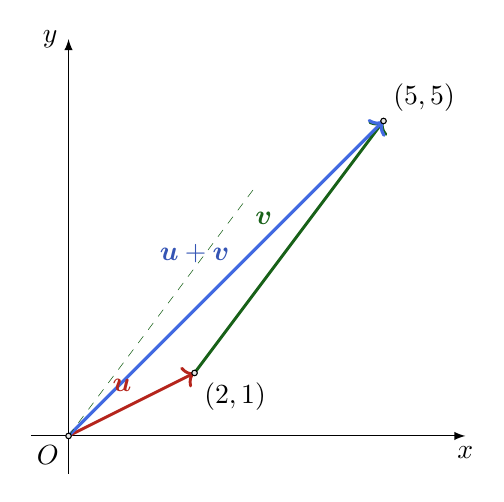
\begin{tikzpicture}[scale=0.8]
  \tkzInit[xmin=-0.6,xmax=5.8,ymin=-0.6,ymax=5.8]
  \tkzDrawX[->]
  \tkzDrawY[->]
  \tkzDefPoint(0,0){O}
  \tkzDefPoint(2,1){U}
  \tkzDefPoint(5,5){S}
  \tkzDefPoint(3,4){V}
  \tkzDrawSegment[->,line width=1.05pt,color=BrickRed](O,U)
  \tkzDrawSegment[->,line width=1.05pt,color=ForestGreen!70!black](U,S)
  \tkzDrawSegment[->,line width=1.15pt,color=RoyalBlue](O,S)
  \tkzDrawSegment[dashed,color=ForestGreen!70!black](O,V)
  \tkzDrawPoints(O,U,S)
  \tkzLabelPoint[below left](O){$O$}
  \tkzLabelPoint[below right](U){$(2,1)$}
  \tkzLabelPoint[above right](S){$(5,5)$}
  \node[text=BrickRed] at (0.85,0.8) {$\vect{u}$};
  \node[text=ForestGreen!70!black] at (3.1,3.45) {$\vect{v}$};
  \node[text=RoyalBlue!80!black] at (2.0,2.9) {$\vect{u}+\vect{v}$};
\end{tikzpicture}
\end{center}

\begin{mathblock}{Theorem}
\begin{theorem}
\[
\begin{bmatrix}
a \\ b
\end{bmatrix}
+
\begin{bmatrix}
c \\ d
\end{bmatrix}
=
\begin{bmatrix}
a+c \\ b+d
\end{bmatrix}.
\]
\end{theorem}
\end{mathblock}

\begin{mathblock}{Proof}
\begin{proof}
The first vector contributes \(a\) horizontally and \(b\) vertically.
The second contributes \(c\) horizontally and \(d\) vertically.

So together the horizontal change is \(a+c\), and the vertical change is \(b+d\).
That is exactly
\[
\begin{bmatrix}
a+c \\ b+d
\end{bmatrix}.
\]
\end{proof}
\end{mathblock}

\begin{mathblock}{Example}
\begin{example}
\[
\begin{bmatrix}
2 \\ 1
\end{bmatrix}
+
\begin{bmatrix}
3 \\ 4
\end{bmatrix}
=
\begin{bmatrix}
5 \\ 5
\end{bmatrix}.
\]
\end{example}
\end{mathblock}

\section{Vectors in Physics}

Now we return to the point from which we started.

\subsection{Velocity}

\begin{problemblock}
If a person walks at \(5\ \mathrm{m/s}\), why is that not enough for a full description?
\end{problemblock}

\begin{solutionblock}
Because \(5\ \mathrm{m/s}\) gives only the magnitude of the motion.
To know the motion itself, we must also know the direction.

So velocity is naturally a vector quantity.
\end{solutionblock}

For instance, if someone walks \(5\ \mathrm{m/s}\) to the east, we may write
\[
\vect{v} =
\begin{bmatrix}
5 \\ 0
\end{bmatrix}\mathrm{m/s}.
\]
If the same person walks \(5\ \mathrm{m/s}\) to the north, we may write
\[
\vect{v} =
\begin{bmatrix}
0 \\ 5
\end{bmatrix}\mathrm{m/s}.
\]

The two vectors have the same magnitude, but they describe different motions.

\begin{center}
\begin{tikzpicture}[scale=0.85]
  \tkzInit[xmin=-0.8,xmax=3.8,ymin=-0.8,ymax=3.8]
  \tkzDrawX[->]
  \tkzDrawY[->]
  \tkzDefPoint(0,0){O}
  \tkzDefPoint(3,0){E}
  \tkzDefPoint(0,3){N}
  \tkzDrawSegment[->,line width=1.1pt,color=BrickRed](O,E)
  \tkzDrawSegment[->,line width=1.1pt,color=RoyalBlue](O,N)
  \tkzDrawPoints(O)
  \tkzLabelPoint[below left](O){$O$}
  \node[text=BrickRed,below] at (1.5,0) {$5\ \mathrm{m/s}$ east};
  \node[text=RoyalBlue,left] at (0,1.5) {$5\ \mathrm{m/s}$ north};
\end{tikzpicture}
\end{center}

\subsection{Displacement}

\begin{problemblock}
A student walks \(4\) meters east and \(3\) meters north.

How should we describe the overall change of position?
\end{problemblock}

\begin{solutionblock}
The displacement is
\[
\vect{d} =
\begin{bmatrix}
4 \\ 3
\end{bmatrix}\mathrm{m}.
\]

Its magnitude is
\[
\lVert \vect{d} \rVert = \sqrt{4^2+3^2}=5.
\]
\end{solutionblock}

This example is simple, but it already shows the power of vectors:
one object records both size and direction.

\subsection{Force}

\begin{problemblock}
Why is force treated as a vector?
\end{problemblock}

\begin{solutionblock}
Because pushing to the right and pushing upward are not the same physical action.

Force must therefore carry direction as well as magnitude.
\end{solutionblock}

\begin{mathblock}{Definition}
\begin{definition}
Force is a vector quantity.
\end{definition}
\end{mathblock}

\begin{mathblock}{Theorem}
\begin{theorem}
Newton's second law may be written in vector form as
\[
\vect{F} = m\vect{a}.
\]
\end{theorem}
\end{mathblock}

This compact formula says, all at once, what happens in every coordinate direction.
That is one reason vectors are so useful in physics: a single vector equation can
stand in place of several ordinary equations.

\section{A Worked Example}

\begin{problemblock}
A force of magnitude \(10\ \mathrm{N}\) acts at an angle of \(30^\circ\) above the horizontal.
Write it as a vector.
\end{problemblock}

\begin{intuitionblock}
The force has one horizontal part and one vertical part.
So we should split it into components.
\end{intuitionblock}

\begin{center}
\begin{tikzpicture}[scale=0.95]
  \tkzInit[xmin=-0.6,xmax=4.5,ymin=-0.6,ymax=2.9]
  \tkzDrawX[->]
  \tkzDrawY[->]
  \tkzDefPoint(0,0){O}
  \tkzDefPoint(3,0){A}
  \tkzDefPoint(3,1.732){F}
  \tkzDrawSegment[->,line width=1.15pt,color=RoyalBlue](O,F)
  \tkzDrawSegment[dashed,color=gray](A,F)
  \tkzDrawSegment[dashed,color=gray](O,A)
  \tkzMarkRightAngle[size=0.22,color=gray](O,A,F)
  \tkzMarkAngle[size=0.45,color=ForestGreen!70!black](A,O,F)
  \tkzLabelAngle[pos=0.75](A,O,F){$30^\circ$}
  \tkzDrawPoints(O,F)
  \tkzLabelPoint[below left](O){$O$}
  \tkzLabelPoint[above right](F){$\vect{F}$}
  \node[below] at (1.5,0) {$F_x$};
  \node[right] at (3,0.85) {$F_y$};
\end{tikzpicture}
\end{center}

\begin{solutionblock}
Its horizontal component is
\[
10\cos 30^\circ = 5\sqrt{3}.
\]

Its vertical component is
\[
10\sin 30^\circ = 5.
\]

Therefore,
\[
\vect{F} =
\begin{bmatrix}
5\sqrt{3} \\ 5
\end{bmatrix}\mathrm{N}.
\]
\end{solutionblock}

\begin{remark}
This is exactly the same idea as before. We take a quantity with direction and rewrite it
in coordinates so that it becomes easier to compute with.
\end{remark}

\section{A Final Theoretical Comment}

At this level, the main theoretical value of vectors is not that they are mysterious.
Quite the opposite: they make things orderly.

\begin{keypointblock}
Vectors help physics for a very simple reason:

\begin{quote}
they let us write one clear law for a quantity that has parts in different directions.
\end{quote}
\end{keypointblock}

For example, the single vector equation
\[
\vect{F}=m\vect{a}
\]
contains the coordinate equations
\[
F_x=ma_x,
\qquad
F_y=ma_y
\]
in the plane.

Thus the vector form is not more complicated than the coordinate form.
In many situations, it is actually cleaner.

\section{Summary}

\begin{enumerate}[label=\arabic*.]
  \item A scalar has magnitude only.
  \item A vector has magnitude and direction.
  \item In the plane, a vector may be written as
  \[
  \begin{bmatrix}
  a \\ b
  \end{bmatrix}.
  \]
  \item Its magnitude is
  \[
  \sqrt{a^2+b^2}.
  \]
  \item Vectors are used in physics for displacement, velocity, acceleration, and force.
  \item Coordinate geometry gives us a very natural way to think about vectors.
\end{enumerate}

\begin{keypointblock}
In the simplest possible words:

\begin{quote}
A vector is a quantity that tells us not only how much, but also which way.
\end{quote}
\end{keypointblock}

\end{document}
